Component diagram mô tả cấu trúc và mối quan hệ giữa các thành phần trong hệ thống theo mô hình \textbf{MVCS}. Để dễ hiểu và quản lý, chúng tôi chia component diagram thành hai loại: \textbf{tổng quan} và \textbf{theo từng vai trò người dùng}.

\subsubsection{Component diagram tổng quan}

\ref{fig:component-overview} minh họa kiến trúc tổng quan của hệ thống, bao gồm frontend người dùng, core backend API, frontend admin, admin backend API, PostgreSQL, Redis cache và các dịch vụ ngoài.

\begin{figure}[htbp]
    \centering
    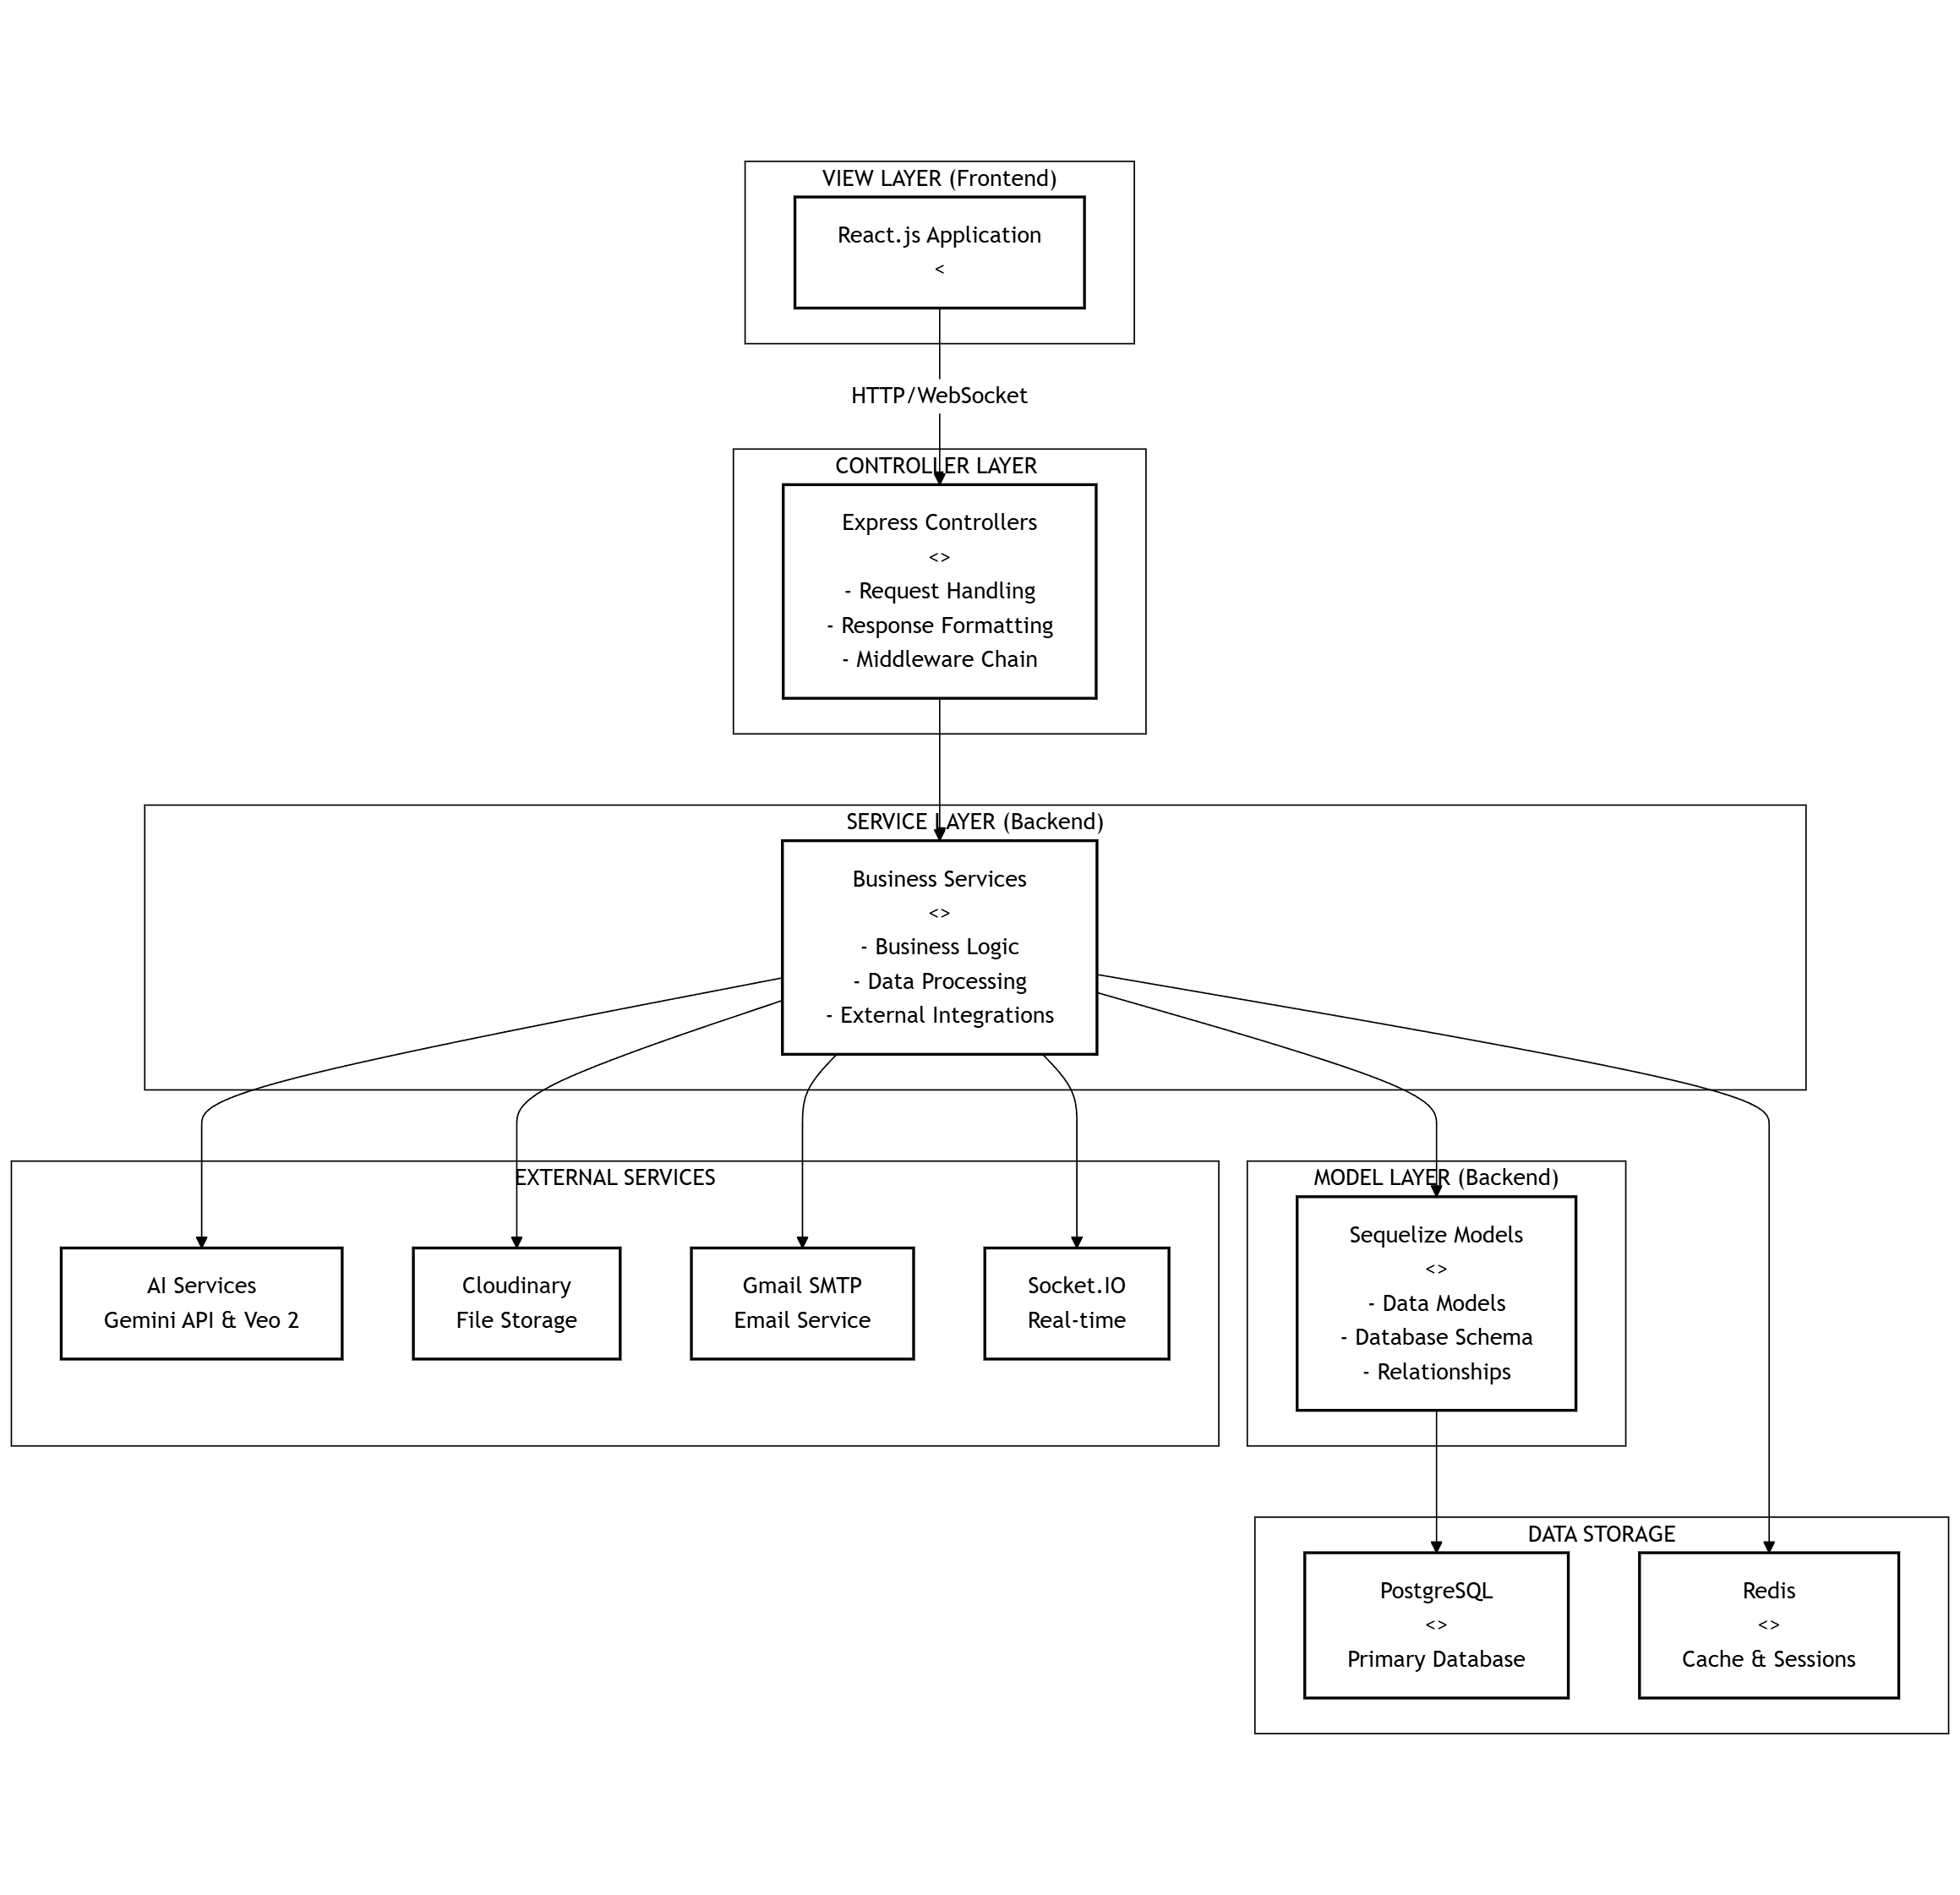
\includegraphics[width=0.9\textwidth]{Images/Component Diagrams/Component Diagram Overview.png}
    \caption{Component Diagram - Tổng quan hệ thống theo MVCS}
    \label{fig:component-overview}
\end{figure}

\paragraph{View Layer (Frontend)} \textbf{View Layer} được xây dựng bằng \textbf{React.js}, \textbf{TypeScript} và \textbf{Vite}, bao gồm:
\begin{itemize}
    \item \textbf{Main Frontend}: Ứng dụng cho buyer/seller/guest, gồm feed, marketplace, cart, checkout, orders, profile, groups, messages, notifications, AI creative lab, AI shopping assistant và seller dashboard.
    \item \textbf{Admin Frontend}: Ứng dụng riêng cho admin, gồm dashboard, users, content, reports, categories, sellers và settings.
    \item \textbf{State \& Context}: Quản lý auth state, notification state, messaging state và các state theo feature.
    \item \textbf{API Services}: Giao tiếp với backend qua REST API bằng fetch wrapper và kết nối Socket.IO cho real-time.
\end{itemize}

\paragraph{Controller Layer (Backend)} \textbf{Controller Layer} được xây dựng bằng \textbf{Express.js}, chịu trách nhiệm:
\begin{itemize}
    \item \textbf{Request Handling}: Nhận và xử lý HTTP request từ frontend.
    \item \textbf{Response Formatting}: Trả response thống nhất cho client.
    \item \textbf{Middleware Chain}: Áp dụng authentication, authorization, validation, rate limiting và error handling.
\end{itemize}

\paragraph{Service Layer (Backend)} \textbf{Service Layer} chứa business logic của hệ thống:
\begin{itemize}
    \item \textbf{Auth \& User Service}: Đăng ký, verify email, login, 2FA, reset password, profile và privacy settings.
    \item \textbf{Social Services}: Feed, posts, likes, comments, follow, saved items, groups và reports.
    \item \textbf{Commerce Services}: Products, variants, cart, orders, refunds, reviews, seller stats và product recommendations.
    \item \textbf{Realtime Services}: Messaging, notification và Socket.IO event emission.
    \item \textbf{AI Services}: Tạo nội dung text, image+text, lưu lịch sử AI, liên kết nội dung với post/scheduled post và cung cấp AI Shopping Assistant qua chatbox.
    \item \textbf{Admin Services}: Quản lý users, content, categories, seller verification và reports.
    \item \textbf{Cache Helper}: Đọc/ghi Redis cho các endpoint đọc nhiều như product list/detail, post list/detail, post comments và search; đồng thời xóa cache liên quan khi dữ liệu bài viết hoặc sản phẩm thay đổi.
\end{itemize}

\paragraph{Model/Data Access Layer (Backend)} \textbf{Model Layer} sử dụng \textbf{Prisma ORM} để:
\begin{itemize}
    \item \textbf{Data Models}: Định nghĩa schema dữ liệu tại \texttt{database/prisma/schema.prisma}.
    \item \textbf{Database Access}: Truy vấn và cập nhật PostgreSQL thông qua Prisma Client.
    \item \textbf{Relationships}: Quản lý quan hệ giữa users, products, orders, posts, groups, messages, notifications, reports và các bảng hỗ trợ.
\end{itemize}

\paragraph{Data Storage \& External Services} Hệ thống sử dụng:
\begin{itemize}
    \item \textbf{PostgreSQL}: Database chính lưu trữ dữ liệu nghiệp vụ.
    \item \textbf{Prisma Client}: Tầng ORM/data access cho backend.
    \item \textbf{Redis}: Cache tùy chọn cho dữ liệu đọc nhiều, được cấu hình bằng \texttt{REDIS\_URL}.
    \item \textbf{Cloudinary}: Lưu trữ và quản lý hình ảnh/file upload.
    \item \textbf{SMTP/Nodemailer}: Gửi email xác thực, OTP và reset password.
    \item \textbf{Socket.IO}: Giao tiếp real-time giữa frontend và core backend.
    \item \textbf{AI Providers}: Gemini cho text/vision; Hugging Face hoặc Replicate cho image generation nếu được cấu hình.
\end{itemize}

\paragraph{MVCS Flow} Luồng xử lý trong hệ thống:
\begin{enumerate}
    \item \textbf{View Layer} gửi request đến backend qua HTTP hoặc kết nối realtime qua Socket.IO.
    \item \textbf{Controller Layer} xác thực, validate và gọi service phù hợp.
    \item \textbf{Service Layer} thực hiện business logic và tương tác với Prisma Client.
    \item \textbf{Prisma Client} truy vấn hoặc cập nhật \textbf{PostgreSQL}.
    \item Với các endpoint đọc nhiều, \textbf{Controller/Cache Helper} có thể lấy dữ liệu từ \textbf{Redis} trước khi gọi service; khi có thay đổi dữ liệu, cache liên quan được invalidation theo pattern.
    \item \textbf{Service Layer} có thể gọi \textbf{Cloudinary}, \textbf{SMTP} hoặc \textbf{AI Providers} khi cần.
    \item Kết quả được trả về frontend; các sự kiện realtime được emit qua Socket.IO.
\end{enumerate}

\subsubsection{Component diagram theo vai trò người dùng}

Để dễ hiểu và phát triển các tính năng cụ thể, chúng tôi chia component diagram thành các diagram theo từng vai trò người dùng trong hệ thống.

\paragraph{Component diagram cho User/Buyer} \ref{fig:component-user-buyer} mô tả các components và flow dành cho người dùng thông thường (User/Buyer).

\begin{figure}[htbp]
    \centering
    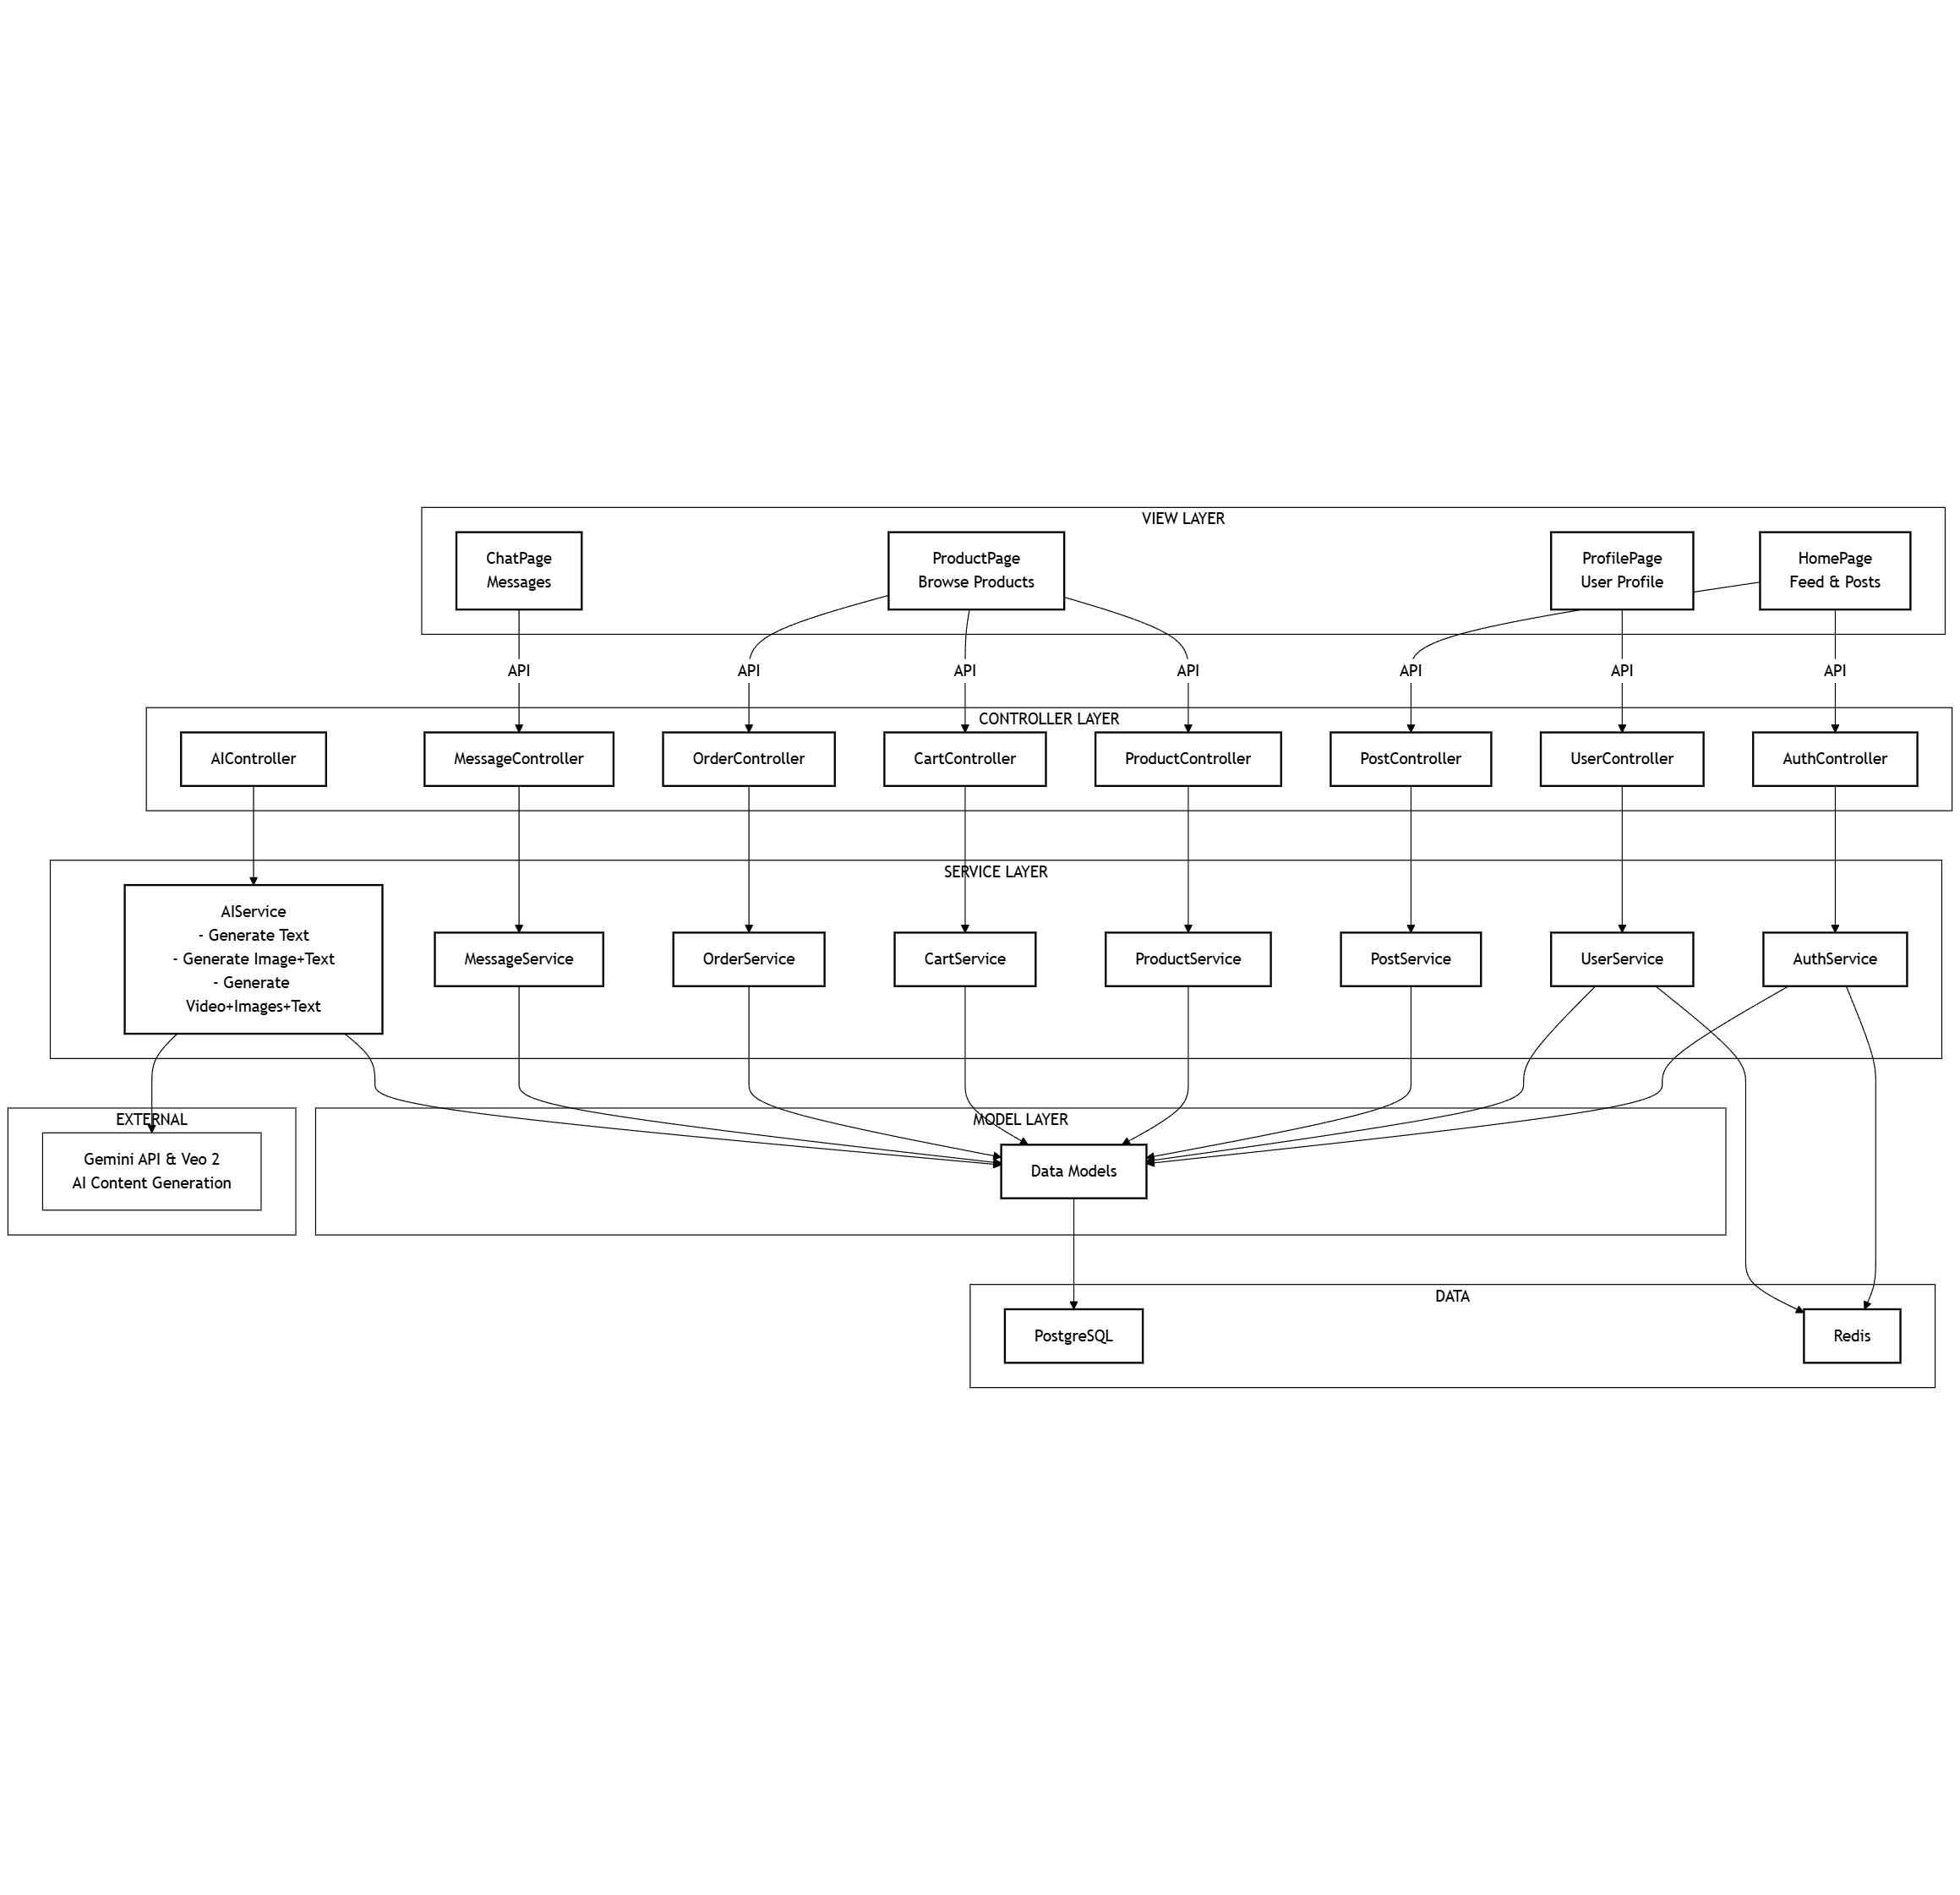
\includegraphics[width=0.9\textwidth]{Images/Component Diagrams/UserBuyer Component Diagram.png}
    \caption{Component Diagram - User/Buyer Role}
    \label{fig:component-user-buyer}
\end{figure}

\textbf{View Layer} bao gồm các trang:
\begin{itemize}
    \item \textbf{Feed/Home}: Trang feed, bài viết và tương tác xã hội.
    \item \textbf{Marketplace/Product Detail}: Duyệt, tìm kiếm, lọc và xem sản phẩm.
    \item \textbf{Cart/Checkout/Orders}: Giỏ hàng, đặt hàng, xác nhận thanh toán và theo dõi đơn.
    \item \textbf{Profile/Saved Items}: Hồ sơ, follow và danh sách đã lưu.
    \item \textbf{Groups/Messages/Notifications}: Nhóm cộng đồng, nhắn tin và thông báo.
\end{itemize}

\textbf{Controller Layer} xử lý các request từ frontend:
\begin{itemize}
    \item \textbf{AuthController, UserController}: Xác thực, profile, follow.
    \item \textbf{PostController, GroupController, ReportController}: Bài viết, nhóm, tương tác và báo cáo.
    \item \textbf{ProductController, CartController, OrderController, ReviewController}: Marketplace, giỏ hàng, đơn hàng và đánh giá.
    \item \textbf{MessageController, NotificationController}: Tin nhắn và thông báo realtime.
\end{itemize}

\textbf{Service Layer} thực hiện business logic tương ứng, còn \textbf{Model Layer} truy cập dữ liệu qua Prisma và PostgreSQL.

\paragraph{Component diagram cho Seller} \ref{fig:component-seller} mô tả các components và flow dành cho người bán (Seller).

\begin{figure}[htbp]
    \centering
    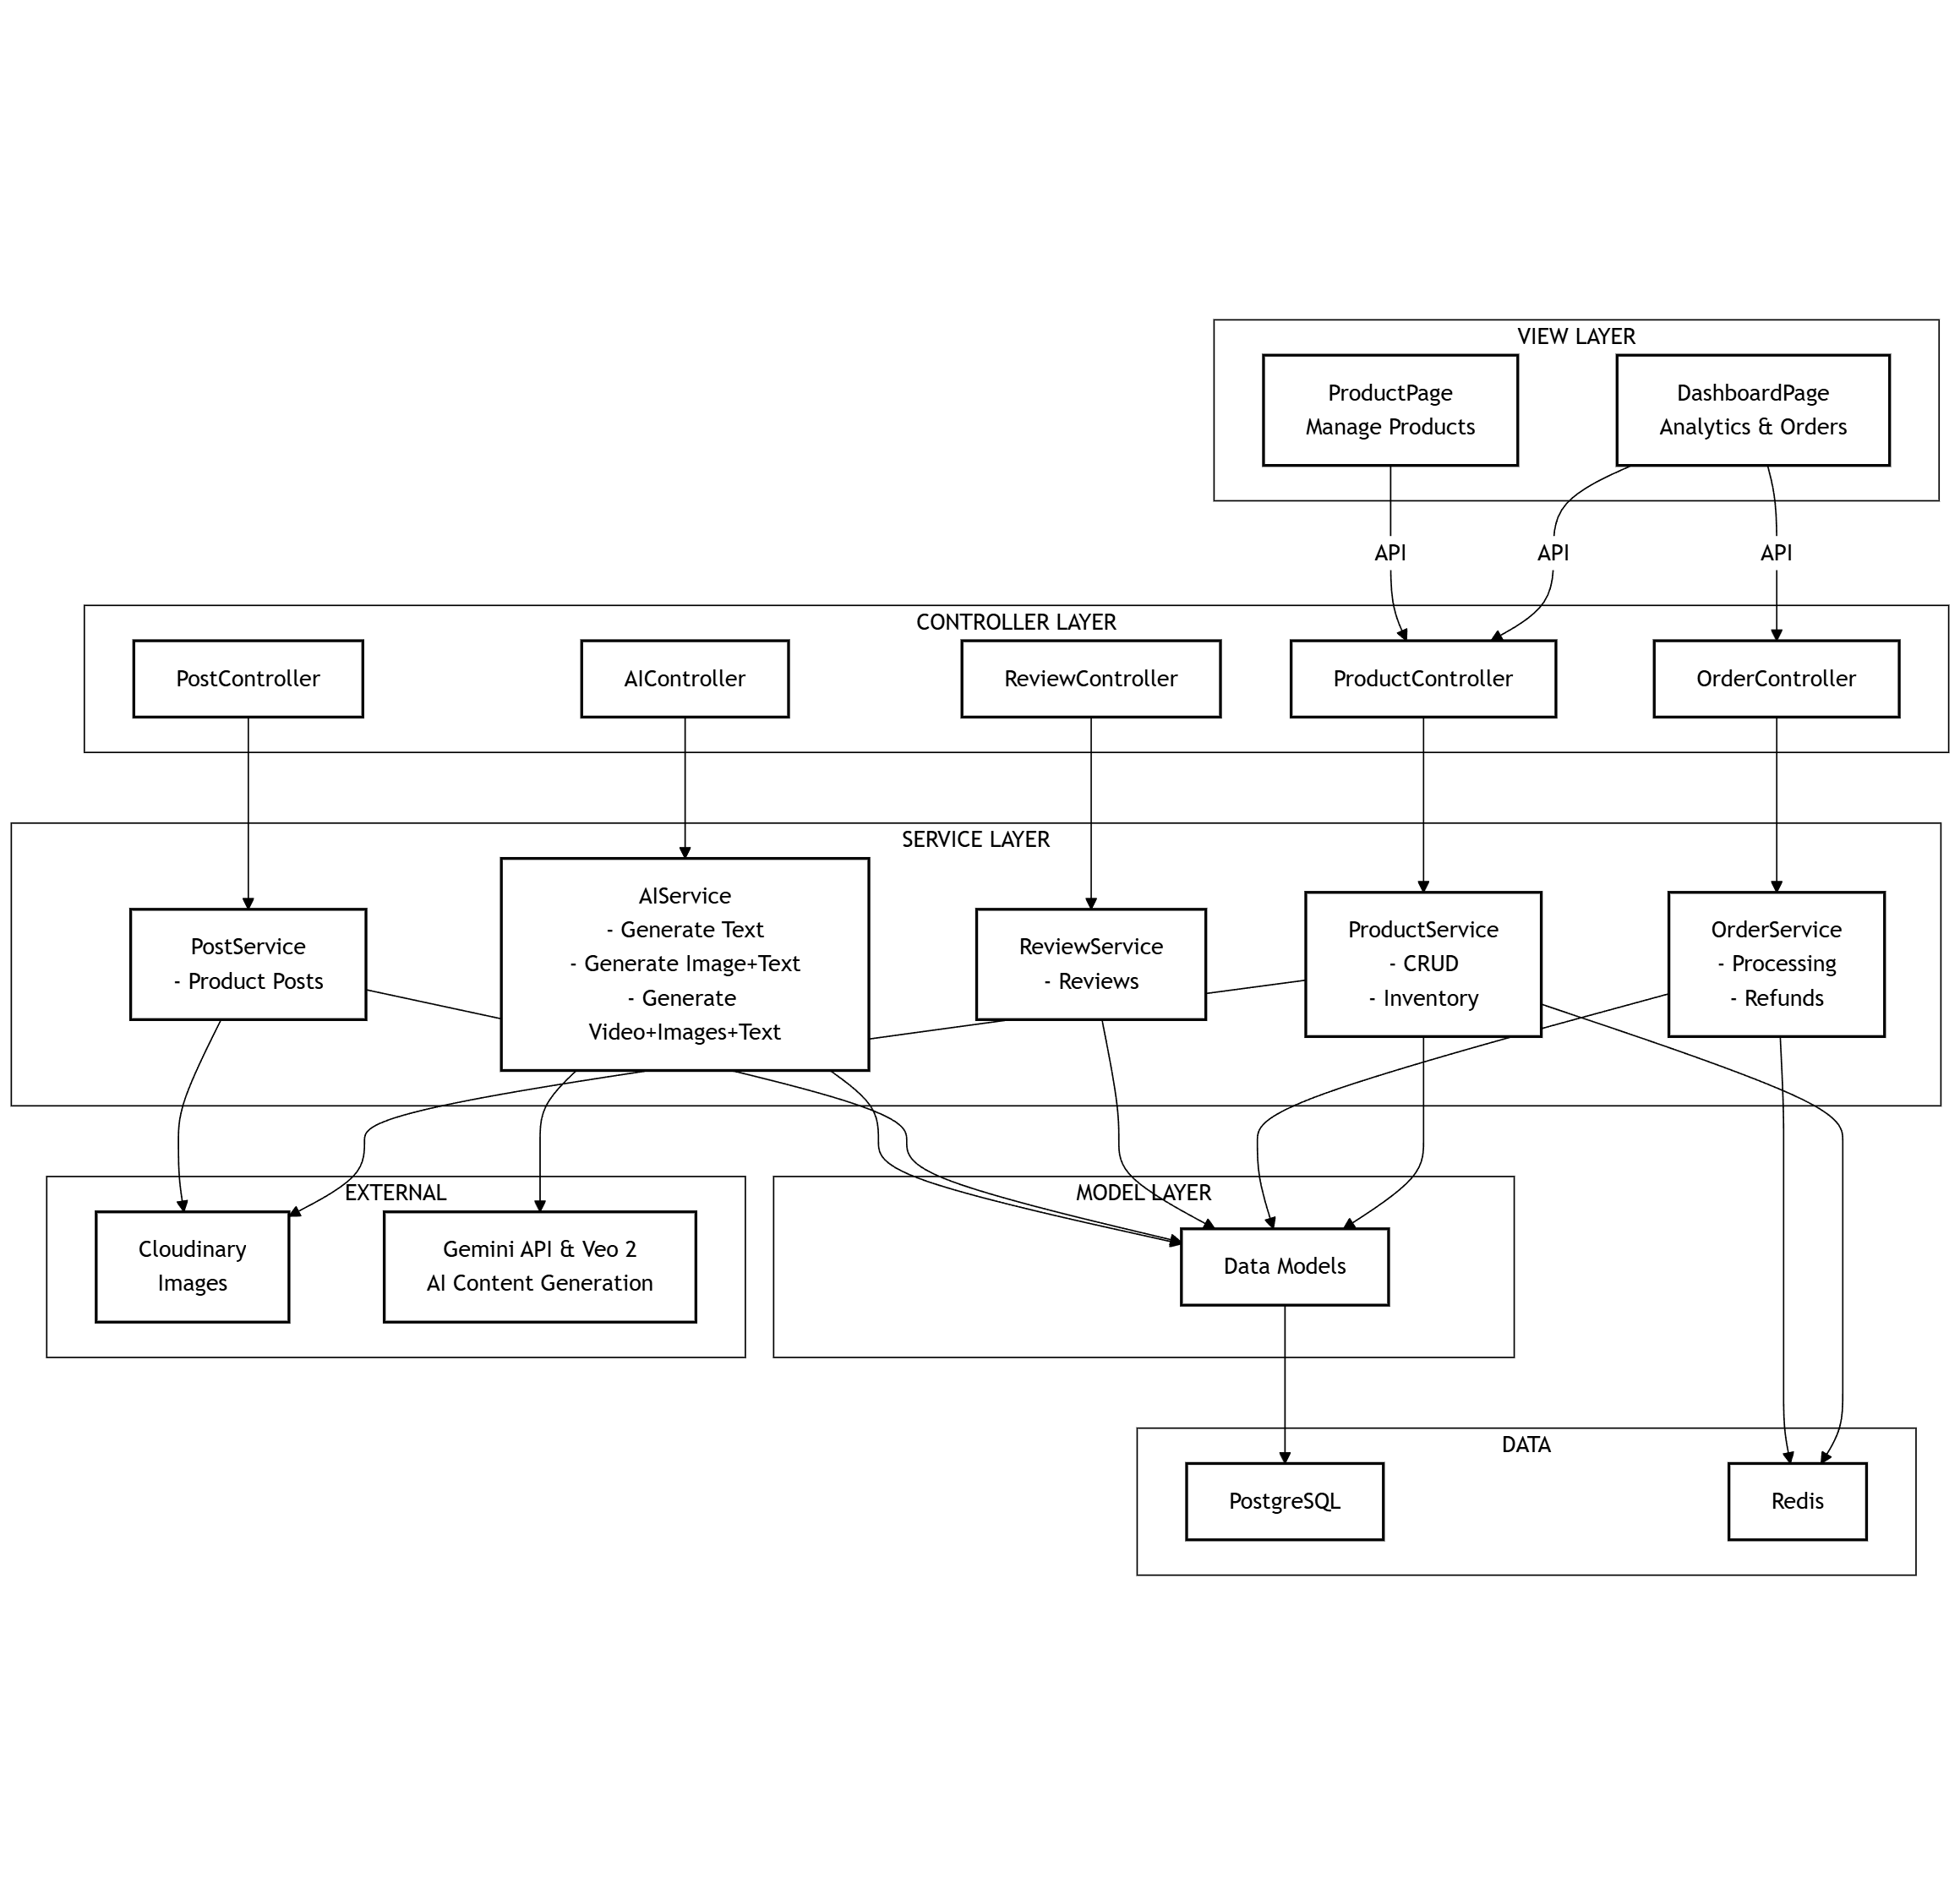
\includegraphics[width=0.9\textwidth]{Images/Component Diagrams/Seller Component Diagram.png}
    \caption{Component Diagram - Seller Role}
    \label{fig:component-seller}
\end{figure}

\textbf{View Layer} cho Seller bao gồm:
\begin{itemize}
    \item \textbf{Seller Registration}: Quy trình đăng ký seller nhiều bước, upload giấy tờ và theo dõi trạng thái duyệt.
    \item \textbf{Seller Dashboard}: Tổng quan doanh thu, đơn hàng, lượt xem và tồn kho.
    \item \textbf{Products/Inventory}: Quản lý sản phẩm, ảnh, biến thể, trạng thái và soft delete/restore.
    \item \textbf{Orders/Refunds/Reviews}: Quản lý đơn bán, xử lý hoàn tiền và phản hồi đánh giá.
    \item \textbf{Scheduled Posts/AI Lab}: Lên lịch bài đăng, tạo nội dung bằng AI và tư vấn mua sắm qua AI chatbox.
\end{itemize}

\textbf{Controller Layer} xử lý các chức năng của Seller:
\begin{itemize}
    \item \textbf{SellerController}: Đăng ký seller, xác minh hồ sơ, sensitive re-auth và change request.
    \item \textbf{ProductController}: Quản lý sản phẩm, inventory và variants.
    \item \textbf{OrderController}: Xem/cập nhật trạng thái đơn hàng và xử lý hoàn tiền.
    \item \textbf{ReviewController}: Phản hồi đánh giá.
    \item \textbf{ScheduledPostController}: CRUD bài đăng đã lên lịch và publish ngay.
    \item \textbf{AIController/AiAssistantController}: Tạo nội dung AI, quản lý lịch sử và xử lý chatbox tư vấn mua sắm.
\end{itemize}

Seller sử dụng \textbf{Cloudinary} để upload ảnh sản phẩm, shop logo/cover và giấy tờ xác minh.

\paragraph{Component diagram cho Admin} \ref{fig:component-admin} mô tả các components và flow dành cho quản trị viên (Admin).

\begin{figure}[htbp]
    \centering
    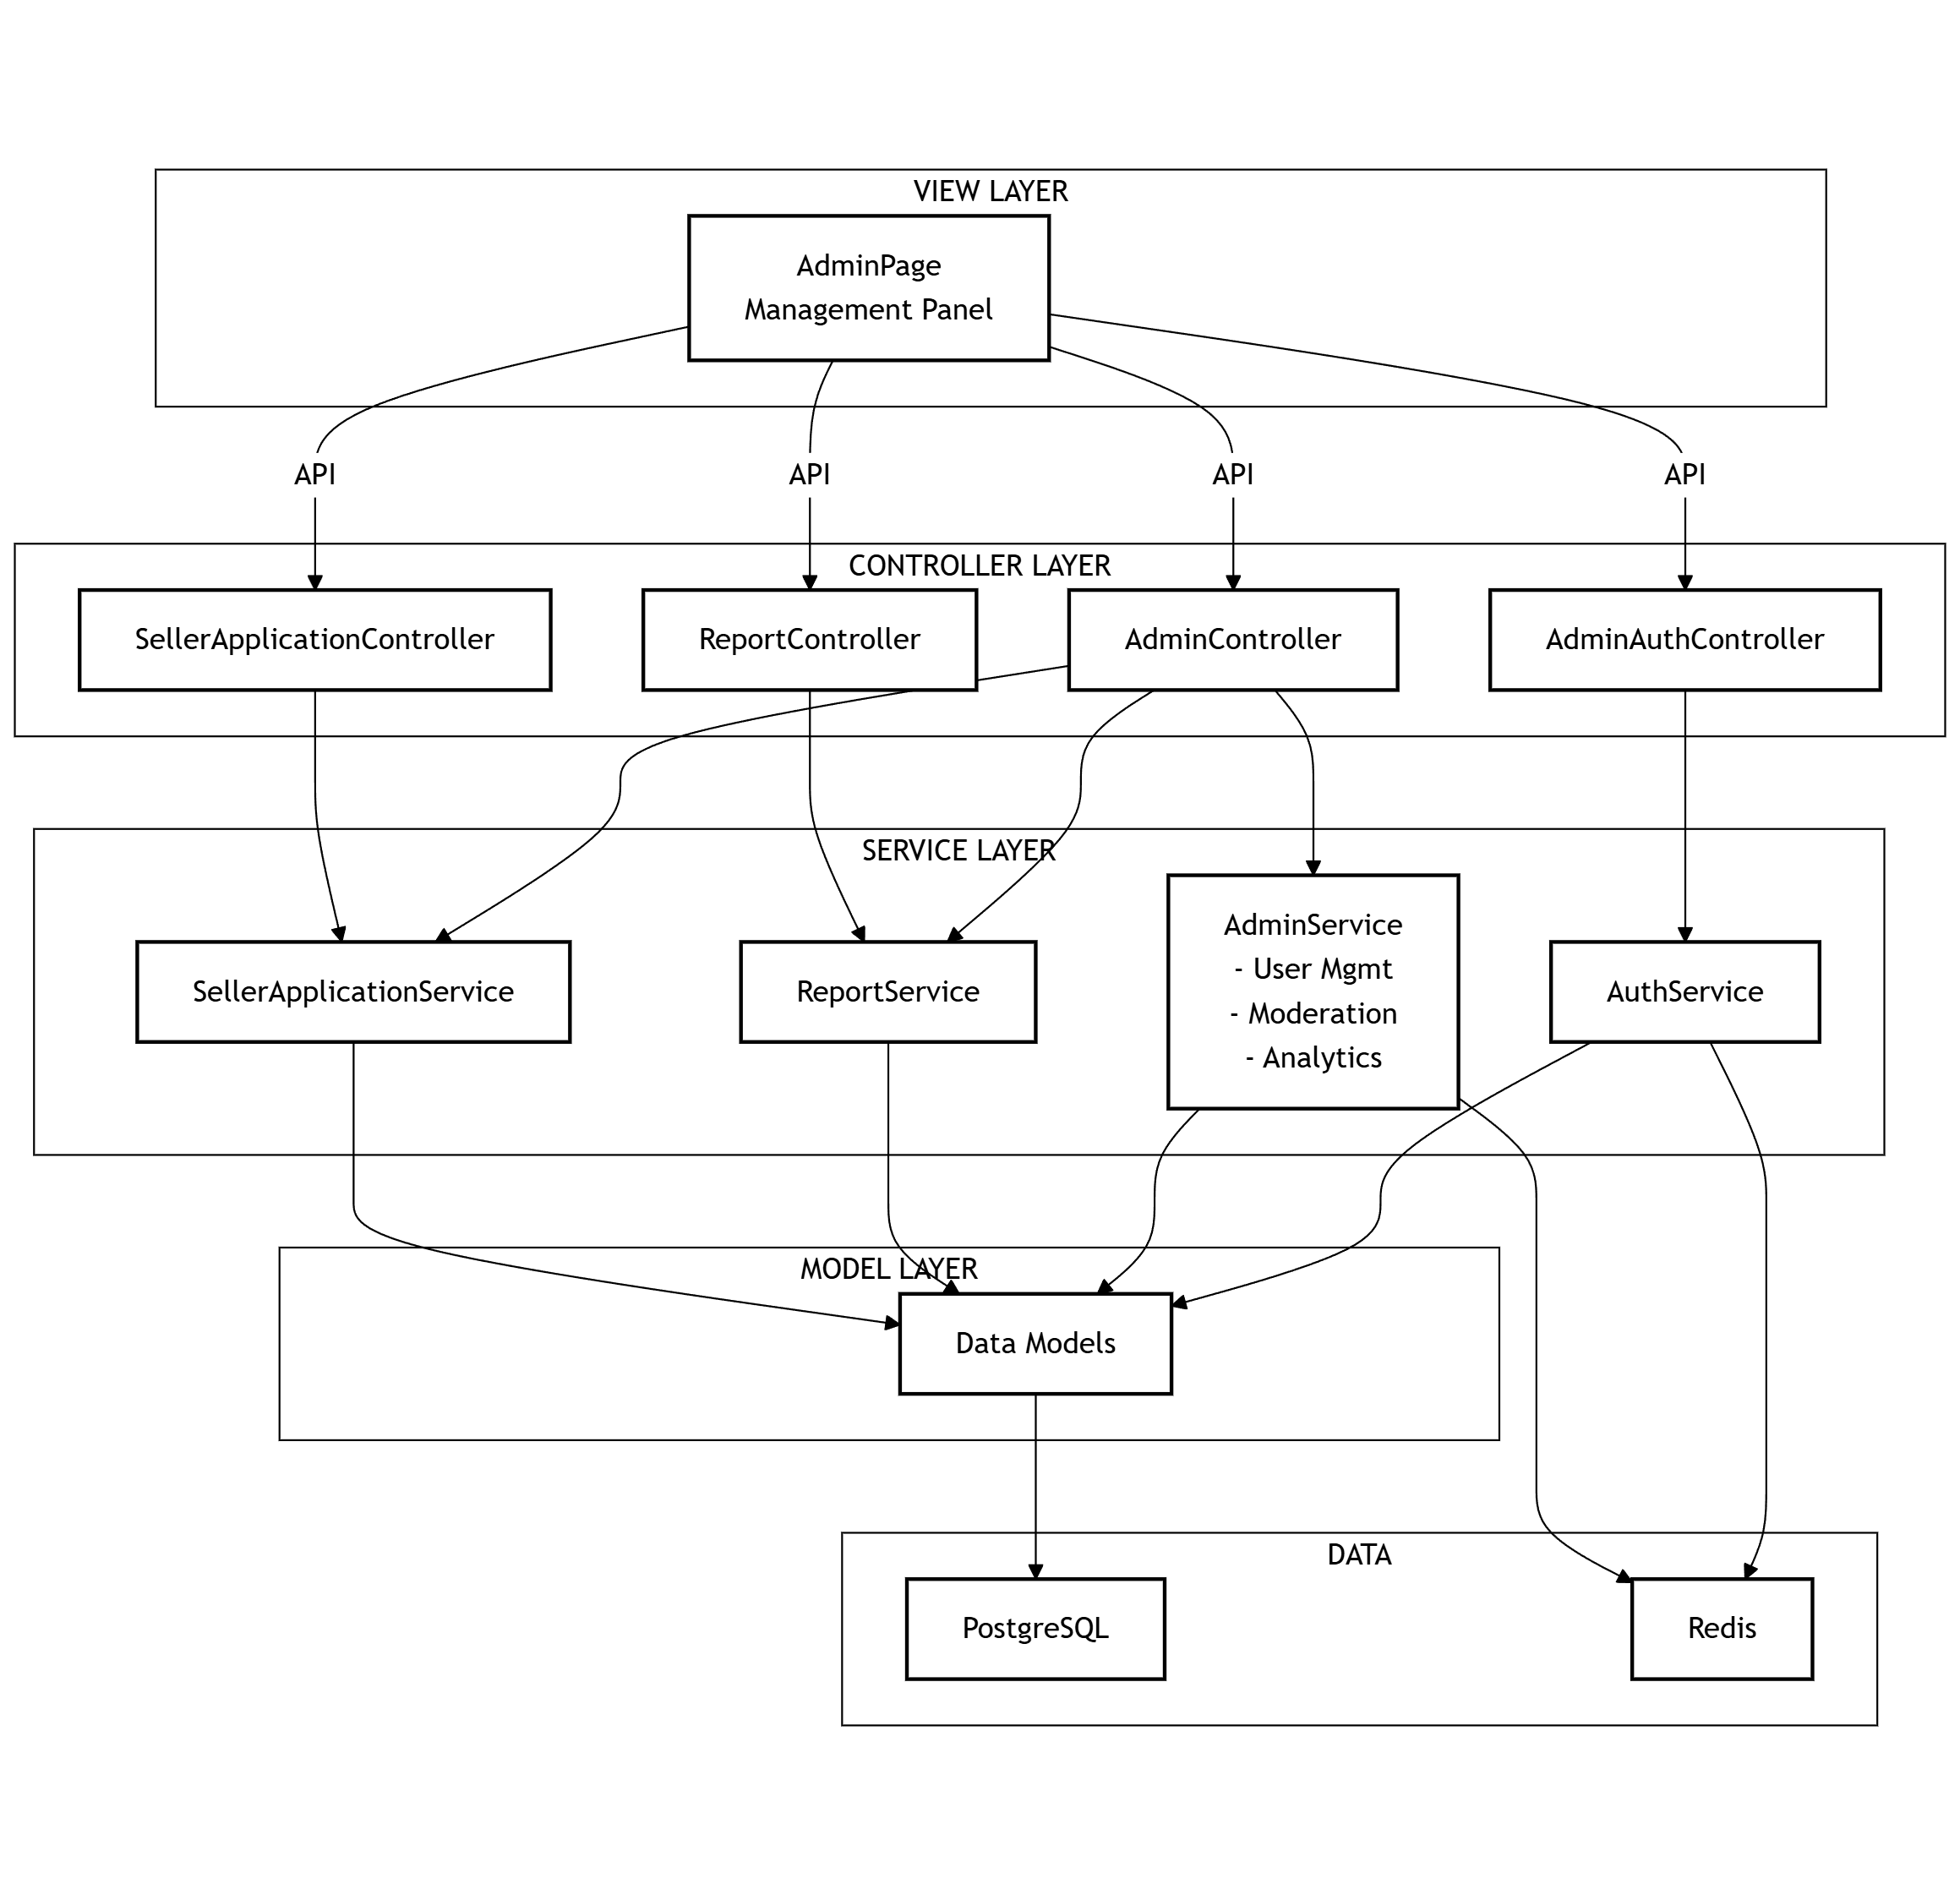
\includegraphics[width=0.9\textwidth]{Images/Component Diagrams/Admin Component Diagram.png}
    \caption{Component Diagram - Admin Role}
    \label{fig:component-admin}
\end{figure}

\textbf{View Layer} cho Admin bao gồm:
\begin{itemize}
    \item \textbf{Admin Login}: Đăng nhập admin qua admin API.
    \item \textbf{Dashboard}: Thống kê tổng quan và growth.
    \item \textbf{Users}: Quản lý user, trạng thái active và role.
    \item \textbf{Content}: Quản lý bài viết và sản phẩm.
    \item \textbf{Reports}: Xem và xử lý báo cáo vi phạm.
    \item \textbf{Categories}: Quản lý danh mục.
    \item \textbf{Sellers}: Duyệt hồ sơ seller và yêu cầu thay đổi dữ liệu nhạy cảm.
\end{itemize}

\textbf{Controller/Service Layer} cho Admin bao gồm:
\begin{itemize}
    \item \textbf{AdminAuthController/AuthService}: Xác thực admin.
    \item \textbf{AdminController/AdminService}: Users, content, categories và dashboard.
    \item \textbf{ReportController/ReportService}: Reports và moderation actions.
    \item \textbf{SellerAdmin Routes/SellerController}: Seller applications và sensitive change requests.
\end{itemize}

\paragraph{Lợi ích của việc chia nhỏ component diagram} Việc chia component diagram thành tổng quan và theo từng vai trò mang lại các lợi ích:
\begin{itemize}
    \item \textbf{Dễ hiểu}: Mỗi diagram tập trung vào một mục đích cụ thể.
    \item \textbf{Dễ maintain}: Cập nhật dễ hơn khi một module thay đổi.
    \item \textbf{Dễ phát triển}: Developers có thể tập trung vào diagram liên quan đến feature đang làm.
    \item \textbf{Dễ tài liệu hóa}: Tài liệu rõ ràng hơn cho từng user type và nhóm chức năng.
\end{itemize}
